\section{Supplementary Identification Diagnostics}

\label{app:fine-F}

The earlier fine-grained panel is retained as an appendix; the three functional groups remain the primary mechanism study. All 21 settings have three actual F seeds, corrected physical-ID IQ binding, fixed default classifiers and seven-view truth-last scores. No old input-invalid scores enter this analysis. All arms share one original F0 G-LU. Their SD is conditional F-seed variation, not independent full-system G variation.

\begin{table*}[t]

\centering\scriptsize

\caption{Completed corrected F diagnostics (accuracy \%, mean$\pm$sample SD). The first row is the reused fixed final T1; every negative contrast remains in the full tables.}

\label{tab:fine-F-complete}

\setlength{\tabcolsep}{3pt}

\begin{tabular}{lp{0.28\textwidth}rrrr}

\toprule

ID & Definition & Raw clean & Raw six views & G-LU clean & G-LU six views \\

\midrule

T1 & Fixed complete final recipe & $84.3944\pm0.9165$ & $70.6013\pm1.0624$ & $84.4839\pm0.9660$ & $77.6468\pm0.8461$ \\

F01 & Shallow-only cross-RX contrast & $84.6153\pm0.9874$ & $70.6531\pm1.3179$ & $84.7006\pm1.0293$ & $77.5923\pm0.7217$ \\

F02 & Intermediate-only cross-RX contrast & $84.4734\pm0.2703$ & $70.7718\pm0.7223$ & $84.5129\pm0.2476$ & $77.8108\pm0.5271$ \\

F03 & Final160-only contrast & $84.6925\pm0.1175$ & $70.6912\pm1.0853$ & $84.7232\pm0.0998$ & $78.1454\pm0.7877$ \\

F04 & No ordinary/raw paired KL & $83.1411\pm0.7607$ & $70.4980\pm0.6128$ & $83.1333\pm0.8212$ & $76.6349\pm0.4797$ \\

F05 & One forward per pair; CE dose retained & $83.7230\pm0.5975$ & $70.7480\pm0.7017$ & $83.7232\pm0.6655$ & $77.2841\pm0.6500$ \\

F06 & One SIG\_TIME view & $84.3780\pm0.6338$ & $70.4099\pm1.1404$ & $84.4470\pm0.6494$ & $77.1662\pm1.1149$ \\

F07 & No signature time coordinates & $84.4127\pm0.4074$ & $70.4179\pm0.7907$ & $84.4829\pm0.4378$ & $77.6429\pm0.4390$ \\

F08 & No signature branch & $82.1323\pm0.5159$ & $68.5587\pm0.2600$ & $82.1927\pm0.5241$ & $73.7291\pm0.7422$ \\

F09 & No PA branch & $81.6974\pm0.4985$ & $63.4471\pm1.1961$ & $81.6893\pm0.5054$ & $75.1410\pm0.4091$ \\

F10 & No reference-response branch & $83.6173\pm0.0918$ & $70.1787\pm0.6468$ & $83.6177\pm0.1073$ & $77.2728\pm0.2800$ \\

F11 & Current student instead of EMA PL source & $84.7266\pm0.1887$ & $70.6681\pm1.0081$ & $84.7893\pm0.2342$ & $77.8307\pm0.2828$ \\

F12 & No adjacent-batch agreement gate & $84.6732\pm0.3554$ & $70.6753\pm0.9747$ & $84.7367\pm0.3898$ & $77.7617\pm0.1711$ \\

F13 & No strong-view agreement gate & $84.6062\pm0.3034$ & $70.6130\pm0.9186$ & $84.6649\pm0.3266$ & $77.7507\pm0.2239$ \\

F14 & No U entropy term & $84.6177\pm0.4434$ & $70.6247\pm0.8817$ & $84.6954\pm0.4750$ & $77.7527\pm0.1944$ \\

F15 & CE + default sat.68; LS0; no SSL/CRIC/KL & $81.5486\pm1.3443$ & $46.3480\pm1.7442$ & $81.4760\pm1.3673$ & $75.0952\pm1.4234$ \\

F16 & CRIC weight zero; other T1 terms retained & $84.7276\pm0.5056$ & $70.9898\pm1.2379$ & $84.7784\pm0.5772$ & $78.0573\pm0.4846$ \\

F17 & As64 replaced by raw64; two CE/KL0 slots & $85.0653\pm0.3262$ & $41.5403\pm4.1600$ & $85.0831\pm0.3053$ & $77.9813\pm0.4494$ \\

F18 & As KL restored to one & $84.6397\pm0.3658$ & $70.9470\pm0.5337$ & $84.6909\pm0.3698$ & $77.9450\pm0.2331$ \\

F19 & No raw pair; CE dose and compute reduced & $84.8135\pm0.4214$ & $71.4128\pm0.9030$ & $84.8841\pm0.4528$ & $78.0841\pm0.5762$ \\

F20 & No U/EMA/entropy; T1 supervision retained & $84.7853\pm0.8236$ & $70.5962\pm0.9519$ & $84.8575\pm0.8694$ & $77.8549\pm0.3960$ \\

F21 & Ordinary PL.95 replacing native SSL; U256 & $84.9817\pm0.1893$ & $70.3594\pm0.9576$ & $85.0296\pm0.2041$ & $78.0746\pm0.1843$ \\

\bottomrule

\end{tabular}

\end{table*}

The diagnostics do not support a claim that every retained element improves every endpoint. F15 is a whole CE-plus-satellite recipe reference with different augmentation, smoothing and exposure. F05 changes stochastic forwards and compute while retaining CE dose; F19 changes both CE dose and compute. F20 removes U from F, but its G-LU readout still uses U through restoration. The separate G-L readouts establish the fully labeled-only boundary.

F17 replaces only the As64 slots by raw64 while retaining their two CE/KL0 slots. Its raw six-view mean is $41.5403\pm4.1600$ versus $70.6013\pm1.0624$ for T1, whereas its restored mean is $77.9813\pm0.4494$. The readout boundary can therefore mask a large raw-view sensitivity; the complete raw and restored tables are retained without target-driven selection.

The 63 corrected F runs total 3150 model epochs, 699300 updates and 189 source stages, or 104.115873 shared-worker hours. The three original final-T1 references reuse 4.617684 historical hours. These are neither incremental deployment latency nor exclusive GPU hours. F15/F20 and the primary factorial reuse some of these sources; panel totals must not be added as disjoint costs.

Every F uses 11100 updates, but F05/F15 evaluate 384 labeled packets per update, F19 evaluates 512, and the other variants evaluate 768. F15/F20 consume zero U; the native-schedule F0 variants each expose 2097900 U packets including final partial batches. F21 ordinary-PL acceptance is 94.8482$\pm$0.1073\% across its three F seeds. Compact native SSL telemetry does not retain a comparable complete acceptance counter; ordinary-PL-only zeros are not interpreted as zero native acceptance.

\begin{figure*}[t]

\centering

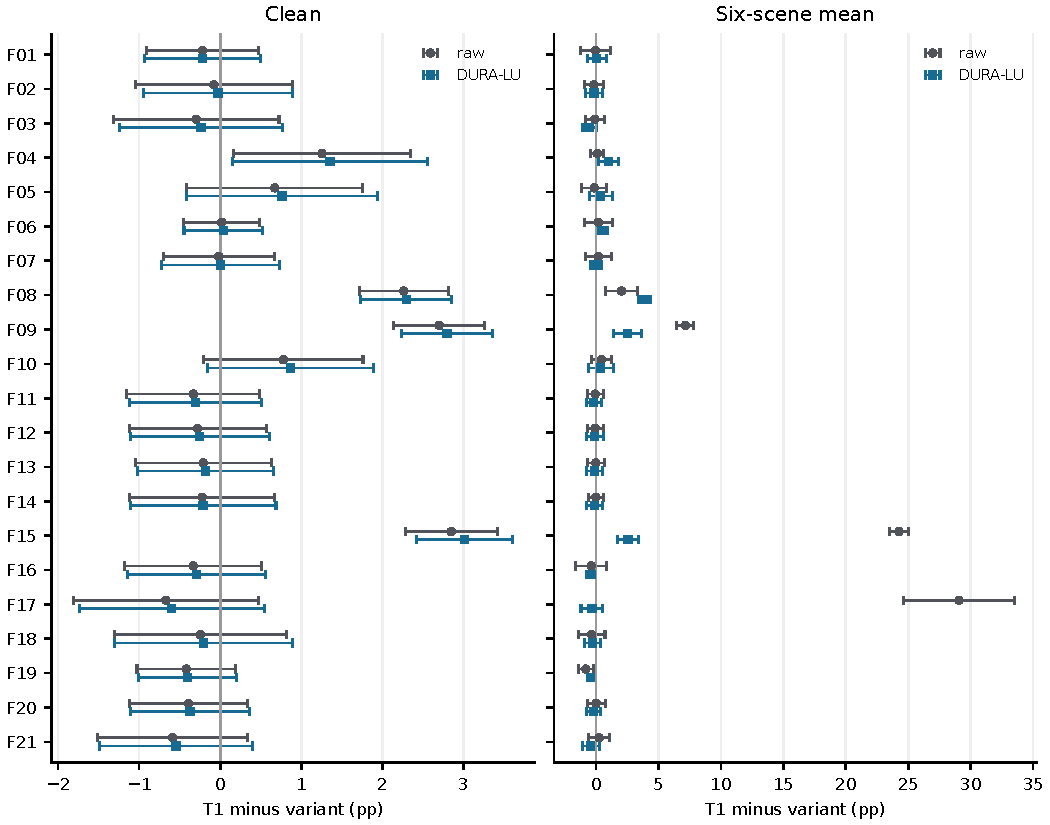
\includegraphics[width=\textwidth]{images/F_ablation63/F_ablation_paired.pdf}

\caption{Fixed-order diagnostic contrasts, full T1 minus each variant (mean$\pm$sample SD of seed-paired differences). Positive values favor T1; all negative values and zero are retained. F15 is a whole-recipe comparator; F05 and F19 also change compute. No arm or endpoint selects a replacement default.}

\label{fig:fine-F-paired}

\end{figure*}

We recomputed 42336 corrected-row confusion matrices, checked 2016 reused T1 reference matrices, and verified 22176 paired correction strata against CM nets and legal joint-count bounds. Full CSVs retain each scene, receiver, transmitter and date, Accuracy/Macro-F1, all paired differences and training cost. Dedicated mechanism timings remain a separate measurement panel; parameter counts and these target accuracies are not speed measurements.
